\section{Determining the effect of $\Delta V_{th}$}
\label{sec:deltavth}

\begin{figure}[thpb]
    \centering
    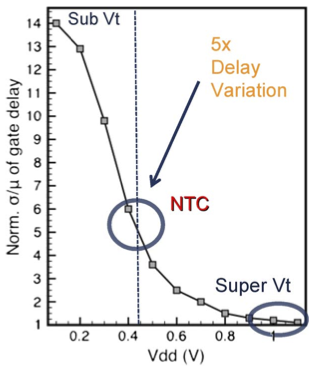
\includegraphics[width=0.4\textwidth]{dreslinski_voltage_delay}
    \caption{Dependence of delay on voltage in near-threshold.~\cite{Dreslinski:2010ez}}
    \label{fig:voltage_delay}
\end{figure}
Because the delay of a gate has a strong dependence on gate voltage in near-threshold operation (see Figure~\ref{fig:voltage_delay}), determining the effect of small changes in $\Delta V_{th}$ is essential to understanding the operation of near-threshold circuits.
This delay is determined by the drain current of the transistor.
The drain current can be described by relatively simple equations for sub threshold \cite{Enz:1995vs} 

\begin{equation}
I_D \propto e^\frac{V_P-V_S}{U_T}
\end{equation}

and super threshold operation

\begin{equation}
I_D \propto (V_P-V_S)^2
\end{equation}

where $V_P=V_G-V_{TH}-\gamma$ with $\gamma$ being a body effect factor. 
For near-threshold operation, however, an interpolation has to be used to bridge these two expressions\cite{Enz:1995vs}, giving us the forward drain current as

\begin{equation}
I_D \propto \left[\ln\left(1+e^\frac{V_G-V_{TH}-\gamma}{2}\right)\right]^2
\end{equation}

This can be related to delay by the equation \cite{Hanson:2007uu}

\begin{align}
t_p &= \frac{k_d\cdot C_L\cdot V_D}{I_{on}}\\
&\propto\frac{V_D}{\left[\ln\left(1+e^\frac{V_G-V_{TH}-\gamma}{2}\right)\right]^2}
\end{align}
 
 
